%%% lorem.tex --- 
%% 
%% Filename: lorem.tex
%% Description: 
%% Author: Ola Leifler
%% Maintainer: 
%% Created: Wed Nov 10 09:59:23 2010 (CET)
%% Version: $Id$
%% Version: 
%% Last-Updated: Tue Oct  4 11:58:17 2016 (+0200)
%%           By: Ola Leifler
%%     Update #: 7
%% URL: 
%% Keywords: 
%% Compatibility: 
%% 
%%%%%%%%%%%%%%%%%%%%%%%%%%%%%%%%%%%%%%%%%%%%%%%%%%%%%%%%%%%%%%%%%%%%%%
%% 
%%% Commentary: 
%% 
%% 
%% 
%%%%%%%%%%%%%%%%%%%%%%%%%%%%%%%%%%%%%%%%%%%%%%%%%%%%%%%%%%%%%%%%%%%%%%
%% 
%%% Change log:
%% 
%% 
%% RCS $Log$
%%%%%%%%%%%%%%%%%%%%%%%%%%%%%%%%%%%%%%%%%%%%%%%%%%%%%%%%%%%%%%%%%%%%%%
%% 
%%% Code:
\chapter{Theory}
\label{cha:theory}
This chapter provides a basic background of the Nordic electricity market, the Swedish electricity market and deep learning (DL). \\
Section \ref{market} describes the Nordic electricity market and the power exchange Nord Pool. Section \ref{DL} introduces artificial neural networks and the main functions behind them. 

\section{The Swedish electricity market and Nord Pool}\label{market}
The Swedish electricity market was deregulated in 1996 which means that it went from being regulated to being exposed to competition \cite{history1}. The Norwegian energy market was also deregulated around the same time, in 1991, where both countries established the power exchange Nord Pool \cite{history2}. Over time, Denmark joined the power exchanged which integrated the Nordic countries into one common Nordic market \cite{history2}. Later in the 2010s, Estonia, Latvia and Lithuania joined Nord Pool following a deregulation as well \cite{history3}. Today, the Nordic market is comprised of Finland, Sweden, Denmark and Norway\cite{history2}. 
\\\\
The Nordic electricity market is divided into the physical market and the financial market \cite{NEM}. The financial market is not relevant to this thesis and will therefore not be discussed here. The physical market consists of the day-ahead market, the intraday market, and the balancing market \cite{NEM}. The scope of this thesis is the day-ahead market where customers can sell or buy energy for the next 24 hours \cite{NordPool} and the intraday market which works together with the day-ahead market to allow same day trading \cite{NordPool_intraday}. Trading on the day-ahead and intraday market is provided by Nord Pool Spot \cite{NEM}. 
\\\\
The Swedish market is divided into four bidding areas as seen in Figure \ref{fig:zones}.
According to Nord Pool, "\textit{the different bidding areas help indicate constraints in the transmission systems, and ensure the regional market conditions are reflected in the price}" \cite{areas}. When there are constraints in the transmission capacity between two bidding areas, power will then transfer from the low price area to the high price area to satisfy the area with the highest demand to prevent bottlenecks \cite{areas}. 

\begin{figure}[H]
    \centering
    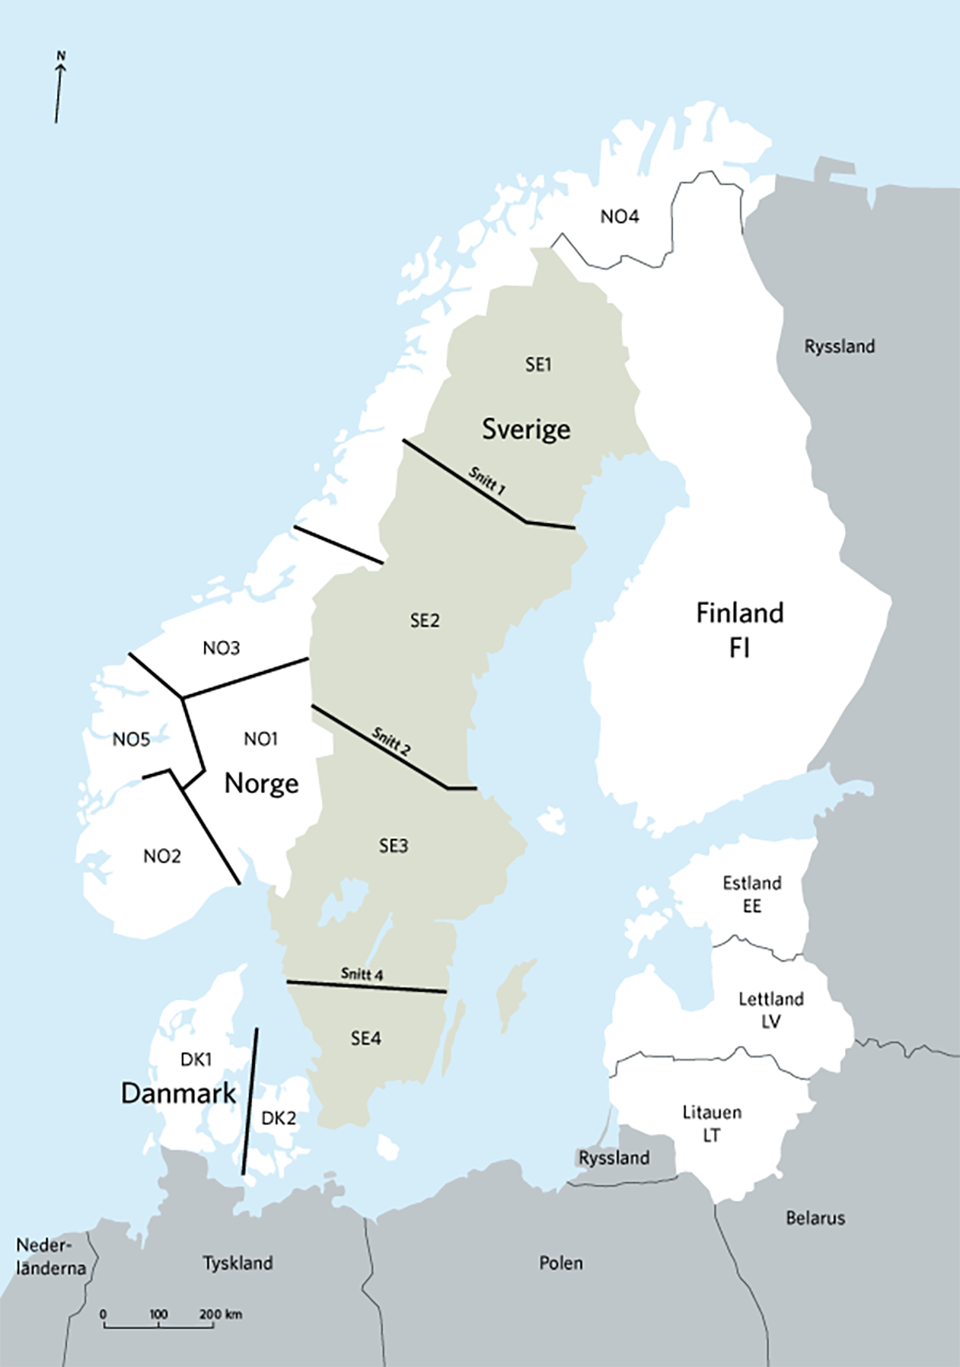
\includegraphics[width=0.5\textwidth]{figures/elomraden.png}
    \caption{Four bidding areas in Sweden}
    \label{fig:zones}
\end{figure}

\noindent
Nord Pool calculates the price for each bidding zone for each hour of the following day based on supply and demand \cite{NordPool} so that equilibrium is expected. For instance, in Sweden the electricity price is lower in the SE1 and SE2 bidding zones compared to SE3 and SE4 bidding zones \cite{areas}. The SE1 and SE2 bidding zones produce more electricity than they consume, which causes electricity to be transported from those zones to SE3 and SE4 \cite{areas}. 

\section{Swedish electricity production}
Electricity in Sweden comes from a variety of energy sources including hydropower, wind power, nuclear power and solar power. Figure \ref{fig:production} shows the distribution of these energy sources in 2023 where the total production was 155 TWh. 

\begin{figure}[H]
    \centering
    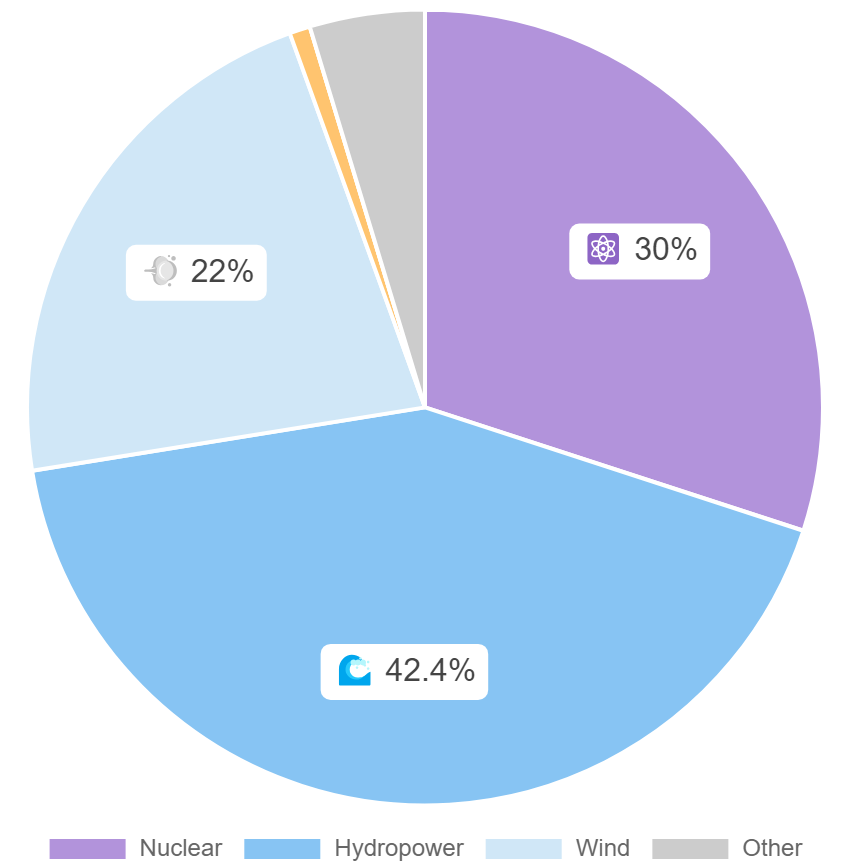
\includegraphics[width=0.5\textwidth]{figures/grossGeneration_2023.png}
    \caption{Electricity generation in 2023 by production type. Orange represents solar power and grey represents other sources such as thermal power \cite{entsoe, lowcarbonpower}.}
    \label{fig:production}
\end{figure}
\noindent
Most of the electricity in the country is generated from low-carbon sources due to large-scale construction of hydropower plants in the early 20th century and the country's commitment to only use low-carbon sources \cite{lowcarbonpower, vattenfall}. Hydropower generated 40.2\% of the total generation followed by nuclear power and wind power with 30\% and 22\%, respectively. In recent years, nuclear power generation has declined due to the closure of two reactors in 2019 and 2020 \cite{energiforetagen}. 

\section{Determinants of electricity price}\label{ch:factors}
The electricity price is mainly based on supply and demand \cite{NordPool}. In case of supply shortage or unusually high demand, the country has an oil-fired condensing power plant that activates as a backup to alleviate the deficit \cite{oilpower}. For instance, the Swedish transmission system operator activated the backup power plant during late 2022 partly because of maintenance of the nuclear power plants and the war in Ukraine \cite{affarsvarlden}. 
\\\\
Due to the variation of energy sources in Sweden, other factors that affect the price are weather conditions where precipitation, temperature and wind impact the production and demand \cite{determinants}, even more so during extreme weather events \cite{spatiotempweather}. On the demand side, seasonal effects such as winter and calendar events such as holidays and weekends are naturally present factors that influence the price in a repeating pattern \cite{WAGNER2022100246}. Naturally, the time of day also affects price.
\\\\
The power generators are also limited by their availability which can change due to planned or unplanned maintenance. Moreover, the different bidding areas, set because of transmission constraints between different regions of the country, also affect the price. Without these constraints, the price would be the same in all four bidding areas \cite{NordPool_capacities}. As an example, Figure \ref{fig:transmission} shows the maximum transmission capacity between the bidding zones assuming no restrictions such as maintenance of power plants in 2021. 

\begin{figure}[H]
    \centering
    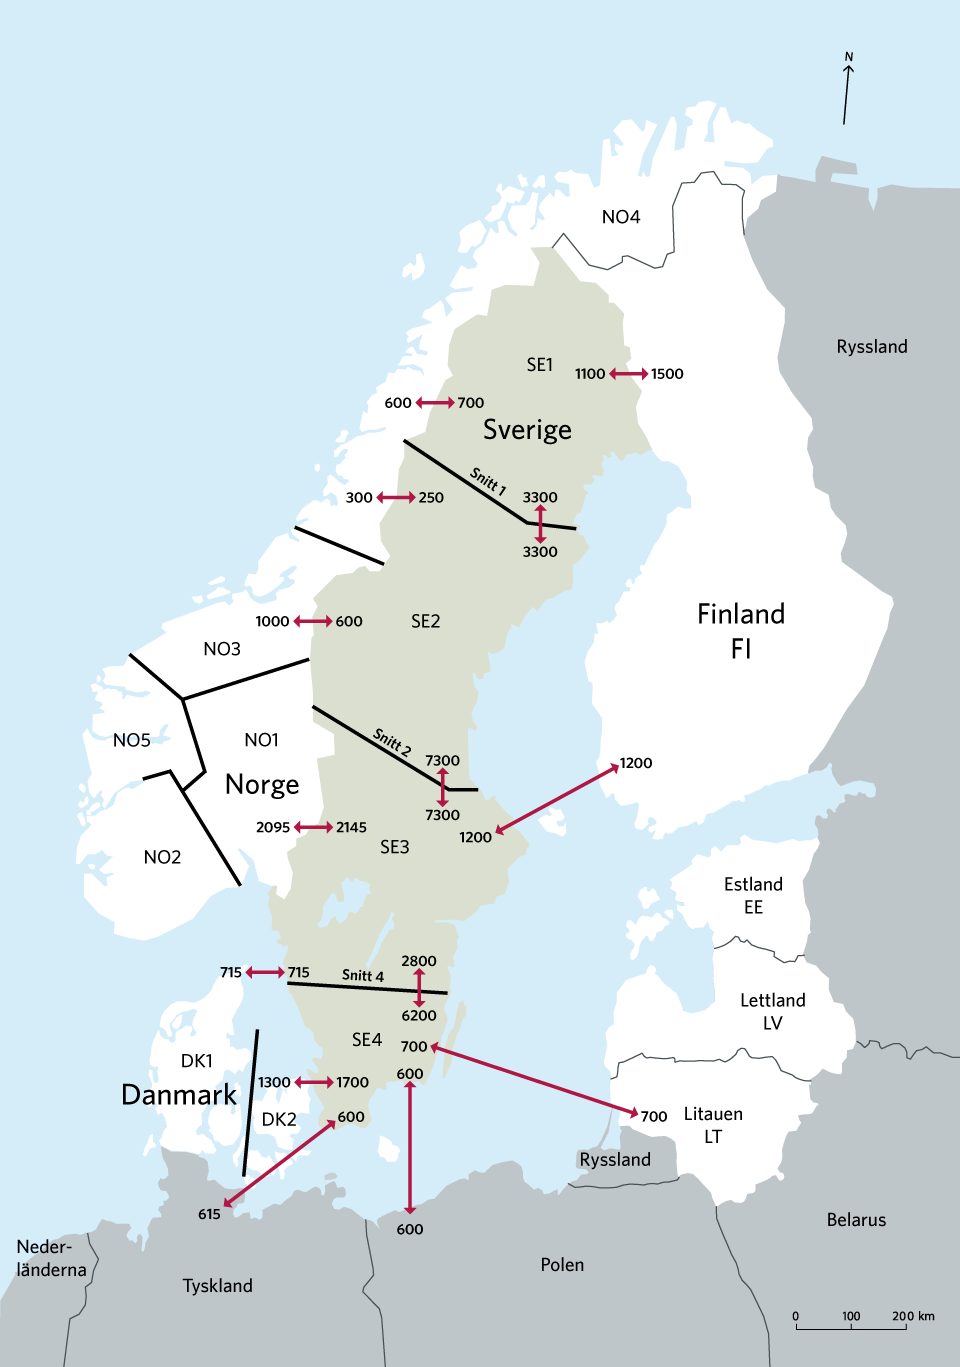
\includegraphics[width=0.6\textwidth]{figures/transmission.png}
    \caption{Maximum transmission capacity between bidding zones as of 2021 \cite{transmission}.}
    \label{fig:transmission}
\end{figure}

The figure shows that electricity flows to and from the bidding zones within Sweden and that the country is also interconnected with Denmark, Norway, Finland, Germany, Poland and Lithuania. This interconnectivity means that the electricity market in Sweden has a direct relationship with those of the other countries\cite{transmission, government_plan}. 

\subsection{Time series forecasting and EPF} \label{timeseriesintro}
%What types of forecasting methods are there, short term/medium term and long term?
%Literature review?

There are different approaches to time series forecasting based on the number of variables and the forecast horizon \cite{multivariate}. A time series is called univariate if it consists of single scalar observations recorder over equal time steps \cite{multivariate}. Multivariate time series extends this notion to include multiple observations, where the idea is to consider the interrelationships and dependencies between these observations \cite{multivariate}. The price of electricity depends on several exogenous factors as described in Section \ref{ch:factors}, which makes EPF a multivariate problem \cite{epf_is_multivariate}. 

When it comes to the forecast horizon, a prediction length of a single time step is known as one-step ahead forecasting \cite{LAGO2021116983, multivariate}. If the prediction length is longer it specifies a multi-step forecasting problem \cite{multivariate}. Moreover, multi-step forecasting can be further divided into short-term and long-term forecasting \cite{multivariate}. While there is no clear consensus as to what threshold defines short term and long term, short term EPF generally implies a forecasting period of minutes up to a few days \cite{LAGO2021116983}. 

The benefits of deep learning in time series forecasting have been heavily used to better model the nonlinear relations between data points and the exogenous factors that drive them \cite{LAGO2021116983}.
\\\\
EPF is a branch of time series forecasting, focusing on the prediction of spot prices on the energy market. Over the last 25 years, there have been various methods applied to EPF from short term to long term. Until the 2010s the field was mostly dominated by early machine learning methods such as linear regression and single-output shallow neural networks \cite{dawn}. As more data and computational power became available the field has seen deeper and more complex networks being applied in EPF research\cite{dawn}.  
\\\\
Neural networks in general are particularly well-suited to EPF as they can learn complex non-linear mappings, which makes them suitable to approximated virtually any type of non-linear relationship that is often found in EPF \cite{goodfellow, dawn}. LSTM, known for its effectiveness in capturing long-range dependencies and temporal patterns \cite{stackedlstm}, has been extensively used in EPF and time series forecasting in general with state-of-the-art results\cite{WAGNER2022100246}.

\section{Artificial Neural Networks and Deep Learning} \label{DL}
While the concept of machine learning has been around since the 1950s, the availability of large amounts of data and computational power made machine learning become more popular during the 2010s in image recognition tasks \cite{dlorigin}. Since then, machine learning has seen promising results across diverse applications including natural language processing, computer vision, and time series forecasting \cite{dlorigin}.

Artificial neural networks (ANNs) are inspired by the biological structure of the brain, and how the neurons in the human brain send signals to each other. ANNs loosely model this behaviour, hence the name. The basic structure of ANNs is organized into layers beginning with an input layer, one or several hidden layers and ending with an output layer as seen in \ref{fig:ann}.
\begin{figure}[H]
    \centering
    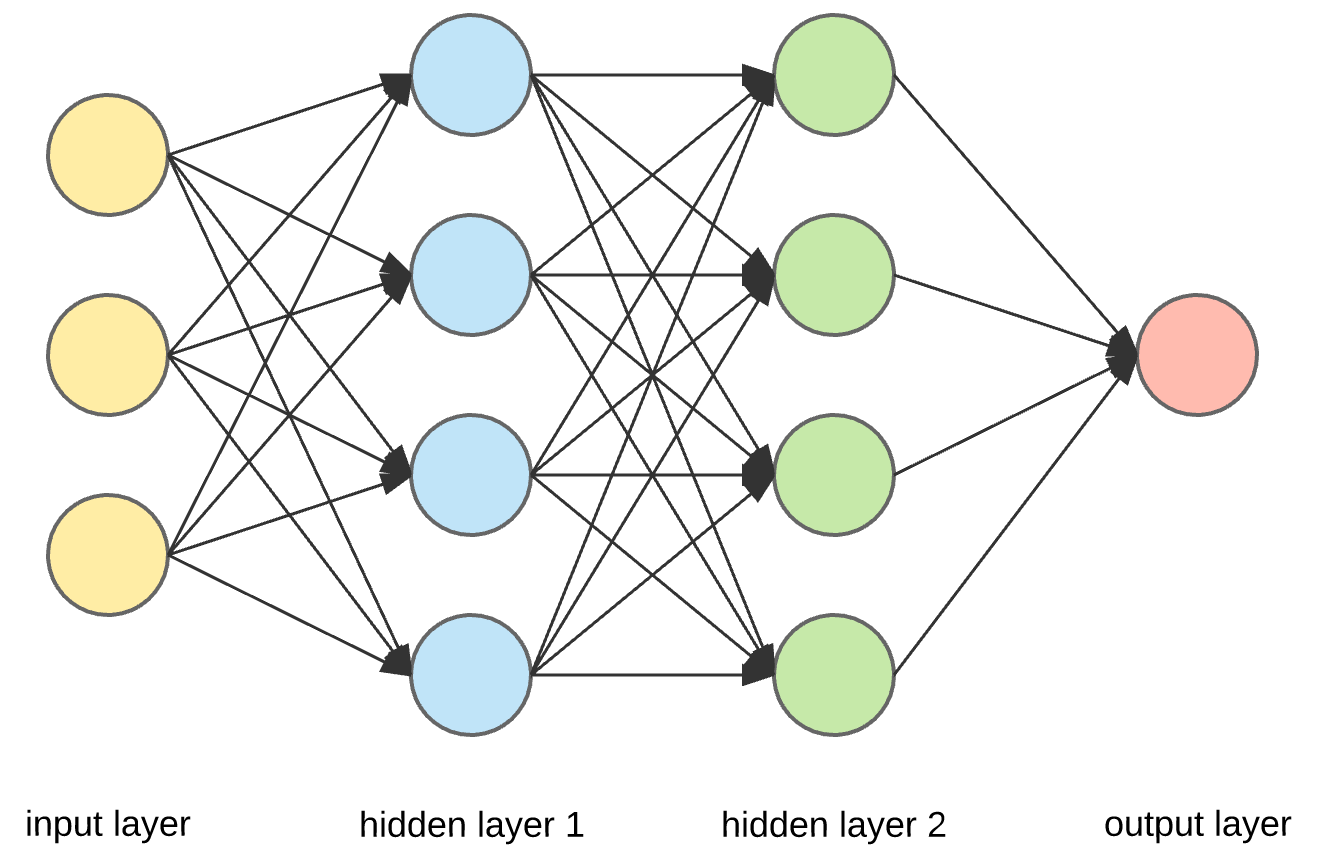
\includegraphics[width=0.5\textwidth]{figures/ann.png}
    \caption{Basic structure of ANNs \cite{medium_figur}}
    \label{fig:ann}
\end{figure}

Each node in an ANN represents a neuron that is connected to another, where the output of one node is sent to other connected nodes in the network. 
The input layer brings the initial data into the network, and the result is produced by the output layer. The hidden layer is the layer that is not directly connected to the input or the output of the network. An ANN with multiple hidden layers in the network is known as deep learning \cite{nielsen}. 
\\
There are different types of ANN architectures applied for different purposes. A deep learning architechture typically consists of several interconnected layers that serve their own purpose. For instance, convolutional layers are known for its many successful applications within computer vision \cite{goodfellow}. 
The simplest type of an ANN is the perceptron. This type of ANN calculates the weighted linear combination of the input and applies an activation function according to \ref{eq:mlp}.
 
\begin{equation} \label{eq:mlp}
    z = \sigma(\sum_{i=1}^{K} {w_{i}x_{i}} + b)
\end{equation}

Where $w \in \mathbb{R}$ is the weight, $b \in \mathbb{R}$ is the bias and $x$ is the input value. Finally, $\sigma$ is the activation function which determines the final output of the neuron depending on its input value and weight. In the case for the perceptron, the activation function is the step function :

\begin{equation} \label{eq:step}
    \sigma(z) =
    \begin{cases}
        1, & \text{if z > 1} \\
        0, & \text{otherwise}.
    \end{cases}
\end{equation}

With multiple layers, Equation \ref{eq:mlp} can be extended to construct a multi-layer perceptron (MLP) where the activation function of neuron $n$ in layer $l$ is determined by \cite{nielsen}:

\begin{equation}\label{eq:mlp2}
    h_{n}^{(l)} = \sigma(\sum_{i=1}^{K} {h_{i}^{(l-1)}w_{n,i}^{(l)} + b_{n}^{(l}}).
\end{equation}

Compared to a single layer perceptron, each hidden layer $l$ in a MLP uses the activation of the previous layer $l-1$ as its input. In MLPs the activation function $\sigma$ is not limited to the step activation meaning different types of activation functions can be used depending on the task \cite{goodfellow}. 
Some activation functions include the rectified linear unit (ReLU) and hyperbolic tangent (tanh) which introduce non-linearity to the network, making it suitable for more complex problems where the relationship between variables are non-linear \cite{goodfellow}. 
\\\\
MLPs are also known as feedforward neural networks (FNNs) which simply means that the information flows only forward from the input layer. The FNN learns by tuning its weights and biases based on a learning algorithm which consists of a loss function and an optimizer. The loss function calculates the difference between the predicted value and the actual value, and the optimizer aims to minimize the difference, i.e the loss. A common optimization approach is the backpropagation algorithm which applies the chain rule for derivatives to calculate the gradient of the loss function for each layer with respect to the weights and biases.

\subsection{Recurrent neural networks and LSTM}
Recurrent neural networks (RNNs) are another type of ANNs. In contrast to FNNs, this network consists of one or more RNN units that loops back on itself, allowing the network to maintain a hidden state that captures information from previous time steps by having an activation function at each time that that is dependent on that of the previous time. Given a vector of input values $\textbf{x}$, the hidden state of the RNN is given by \cite{rnnHiddenState}:

\begin{equation} \label{eq:hiddenStateRNN}
    h_{t} = 
    \begin{cases}
        0, & \text{t = 0} \\
        \phi(h_{t-1}, x_{t}), & \text{otherwise}.
    \end{cases}
\end{equation}
Where $\phi$ is a non-linear function. A common implementation of Eq. \ref{eq:hiddenStateRNN} is: 

\begin{equation}\label{eq:vanilla-rnn}
    h_{t} = \sigma(W_{x}x_{t} + W_{h}h_{t-1} + b_{h}).
\end{equation}

Where $W_{x}$ and $W_{h}$ are weight parameters, $x_{t}$ is the input vector and $h_{t-1}$ is output of the hidden state from the previous time step $t$. Finally, $\sigma$ is a non-linear activation function, such as tanh. This allows the network to memorize information as it learns, making it more specialized towards sequenced data such as time series. 
\\\\
One drawback of RNN is the vanishing gradient problem, which means that the networks gradient approaches zero during backpropagation\cite{LSTM}. This causes the RNN to fail in learning properly from the data and the risk of the problem increases with more layers in the network \cite{diveLSTM}. Similarly to the vanishing gradient, RNN also suffer from exploding gradients where the gradient increases exponentially which causes the network to become unstable \cite{LSTM}.
\\\\
To deal with this drawback, Hochreiter and Schmidhuber \cite{LSTM} have developed Long-short term memory (LSTM). The structure of a LSTM cell is shown in \ref{fig:lstm-cell}. 

\begin{figure}[H]
    \centering
    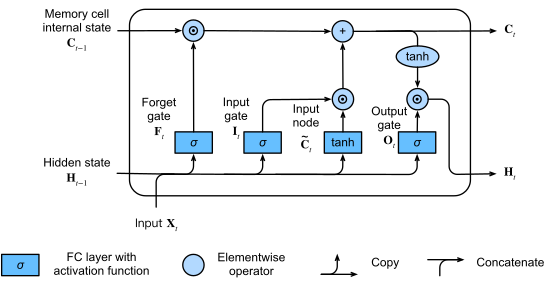
\includegraphics[width=0.7\textwidth]{figures/lstm_cell.png}
    \caption{The LSTM cell \cite{diveLSTM}.}
    \label{fig:lstm-cell}
\end{figure}

LSTM is a type of RNN that leverages a gating mechanism to selectively update the network at each step. To do this, a LSTM cell contains three gates: the input gate $I_{t}$, the forget gate $F_{t}$ and the output gate $O_{t}$, as shown in Figure \ref{fig:lstm-cell} \cite{diveLSTM}. Additionally, the LSTM cell also includes the internal state $C_{t-1}$ which acts as a long-term memory, hidden state $h_{t-1}$ which acts as a short-term memory and the memory cell $C_{t}$. \\

Unlike the RNN implementation described in Equation \ref{eq:vanilla-rnn}, a LSTM cell maintains a memory. This means that the hidden state is calculated by:

\begin{equation}
    h_{t} = O_{t}tanh(C_{t}).
\end{equation}

Where tanh is the activation function for $C_{t}$ that lies in the range $(-1,1)$ $O_{t}$ is the output gate which is calculated by:

\begin{equation}\label{eq:ogate}
    O_{t} = \sigma(W_{O}x_{t} + U_{O}h_{t-1} + b_{O}),
\end{equation}

where $W_{f}$ and $U_{O}$ are the weight parameters, $x_{t}$ is the input value and $h_{t-1}$ is the hidden state of the previous time step. $\sigma$ is the sigmoid function given by:

\begin{equation}\label{eq:sigmoid}
    \sigma(x) = \frac{1}{1+e^{-x}}.
\end{equation}

Correspondingly, the forget gate and the input gate are calculated as follows:

\begin{equation}\label{eq:figate}
    \begin{aligned}
    F_{t} = \sigma(W_{F}x_{t} + U_{F}h_{t-1} + b_{F}) \\
    I_{t} = \sigma(W_{I}x_{t} + U_{I}h_{t-1} + b_{I}).
    \end{aligned}
\end{equation}
Due to the sigmoid activation function in Equation \ref{eq:sigmoid}, the resulting values of the three gates \ref{eq:ogate} \& \ref{eq:figate} are in the range $(0,1)$
The reasoning for the three gates provides LSTM the ability to determine whether what information will be retained or not over a long sequence, capturing important features from the data long-term \cite{diveLSTM}.\\
The memory cell is calculated in a similar fashion to the three gates described above, but uses a tanh as the activation which leads to:

\begin{equation}
    \hat{C_{t}} = tanh(W_{c}x_{t} + U_{c}h_{t-1} + b_{c})
\end{equation}

where $W_{c}$ and $U_{c}$ are weight parameters and $b_{c}$ is the bias. The input gate $I_{t}$ determines how much of the input $x_{t}$ is combined via the input node $\hat{C_{t}}$, while the forget gate $F_{t}$ determines how much of the internal state $C_{t-1}$ is added to the output. The update equation combining these components is given by:

\begin{equation}
    C_{t} = F_{t} \odot C_{t-1} + I_{t} \odot \hat{C_{t}}.
\end{equation}

Due to the additive update equation and the gating mechanism, LSTM networks are able to decide the flow of information and thus the gradient by preventing irrelevant information from accumulating or important information from fading \cite{LSTM}. The three gates also control how the gradients are affected by the input and the output from the previous time step which helps alleviate the vanishing and the exploding gradient problems \cite{diveLSTM}. 

\subsection{Modeling approaches}
As described in Section \ref{timeseriesintro}, there are different types of time series problems depending on the number of variables and the forecast horizon. Consequently, there are also different ways to design models depending on the time series problem. Classical time series models aim to predict the target time series $y_{t+1}$ given its historical values $y_{t} = (y_{t}, y_{t-1}, ... , y_{0})$ \cite{mqrnn}. However, time series problems such as EPF is far more complex where many covariates are present \cite{mqrnn}. Furthermore, covariates can be differentiated depending on whether they are known in advance or not \cite{darts}. In the context of EPF, covariates include production data, consumption data and seasonality. Both production and consumption data are examples of past covariates, which are observed covariates only known into the past. In contrast, seasonality generally consists of predictable patterns such as the hour of the day and the day of the week. Such information is known into the future, and can include covariates such as weather forecasts which are predicted with reasonable accuracy \cite{smhiprognos}. A common modeling approach to incorporate both past and future covariates is known as sequence-to-sequence modeling. First introduced in 2014 by Graves \cite{graves}

\subsubsection{Sequence to sequence modeling}
Sequence to sequence modeling is a modeling approach that is flexible 

%%%%%%%%%%%%%%%%%%%%%%%%%%%%%%%%%%%%%%%%%%%%%%%%%%%%%%%%%%%%%%%%%%%%%%
%%% lorem.tex ends here

%%% Local Variables: 
%%% mode: latex
%%% TeX-master: "demothesis"
%%% End: 
